\def\tutdate{12.01.2017}
\ifdefined\compileall \else
\ifdefined\compiletype
	\documentclass[handout]{beamer}
\else
	\documentclass{beamer}
	\def\compiletype{livebeamer}
\fi

\usepackage{templates/beamerthemekitwide}

\usepackage[utf8]{inputenc}
\usepackage[T1]{fontenc}
\usepackage[ngerman]{babel}
\usepackage{listings}
\usepackage{hyperref}
\usepackage{graphicx}

\usepackage{amsmath}
\usepackage{amsthm}
\usepackage{amssymb}
\usepackage{polynom}

\usepackage{ifthen}
\usepackage{adjustbox} % for \adjincludegraphics

\newcommand{\markBlue}[1]{\textcolor{kit-blue100}{#1}}
\newcommand{\markGreen}[1]{\textcolor{kit-green100}{#1}}

\newcommand{\pitem}{\pause\item}
\newcommand{\p}{\pause}

% -- MATH MACROS
\newcommand{\thistheoremname}{}
\newcommand{\G}{\mathbb{Z}}
\newcommand{\B}{\mathbb{B}}
\newcommand{\R}{\mathbb{R}}
\newcommand{\N}{\mathbb{N}}
\newcommand{\Q}{\mathbb{Q}}
\newcommand{\C}{\mathbb{C}}
\newcommand{\Z}{\mathbb{Z}}
\newcommand{\F}{\mathbb{F}}
\newcommand{\mi}{\mathrm{i}}
\renewcommand{\epsilon}{\varepsilon}


\newenvironment<>{taskblock}[1]{%
	\setbeamercolor{block title}{fg=kit-orange15,bg=kit-orange100}
	\setbeamercolor{block body}{fg=black,bg=kit-orange30}%
	\begin{block}#2{#1}}{\end{block}}

\setbeamertemplate{enumerate items}[default]

% Aussagenlogik Symbole
\newcommand{\W}{w}
\renewcommand{\F}{f}

% Kodierung
\newcommand{\frepr}{\textbf{repr}}
\newcommand{\fRepr}{\textbf{Repr}}
\newcommand{\fZkpl}{\textbf{Zkpl}}
\newcommand{\fbin}{\textbf{bin}}
\newcommand{\fdiv}{\textbf{ div }}
\newcommand{\fmod}{\textbf{ mod }}

\title[Grundbegriffe der Informatik]{Grundbegriffe der Informatik\\Tutorium 33}
\subtitle{}
\author{Lukas Bach, lukas.bach@student.kit.edu}
\date{\tutdate}

\institute{}

\titlelogo{lukasbach}

\titleimage{bg}
%\titleimage{bg-advent}


\ifthenelse{\equal{\compiletype}{livebeamer}}
	{
		\def\livebeamermode{1}
	}{}

\ifthenelse{\equal{\compiletype}{print}}
	{
		\def\printmode{1}
	}{}

\setbeamercovered{invisible}

%\usepackage[citestyle=authoryear,bibstyle=numeric,hyperref,backend=biber]{biblatex}
%\addbibresource{templates/example.bib}
%\bibhang1em

\begin{document}
	
\selectlanguage{ngerman}


%title page
\begin{frame}
	\titlepage
\end{frame}

%table of contents
\ifdefined\printmode
	\ifdefined\compileall \else
	\begin{frame}{Gliederung}
		\tableofcontents
	\end{frame}
\fi\fi

\fi

\section{Graphen}
\begin{frame}{Graphen}
	\begin{block}{Definition: Graph}
		\ip Ein Graph $G = (V,E)$ ist ein Tupel aus:
		\begin{itemize}
			\pitem Einer endlichen, nichtleeren Knotenmenge $V$
			\pitem Einer endlichen Kantenmenge $E \subseteq V \times V$
		\end{itemize}
	\end{block}
	
	\bp
	
	Beispiel: Knotenmenge $V := \{a, b, c, d\}$. Kantenmenge könnte zum Beispiel sein...
	
	\begin{itemize}
		\pitem $E := \{(a,b), (c, d), (a, d)\}$
		\pitem $E := \{(a,a), (b,b), (c,c)\}$
		\pitem $E := \emptyset$
	\end{itemize}
\end{frame}

\begin{frame}{Wie sehen diese Graphen aus?}
	Beispiel: Knotenmenge $V := \{a, b, c, d\}$. Kantenmenge könnte zum Beispiel sein...
	\begin{itemize}
		\pitem $V := \{a, b, c, d\}, E := \{(a,b), (c, d), (a, d)\}$\\
		\p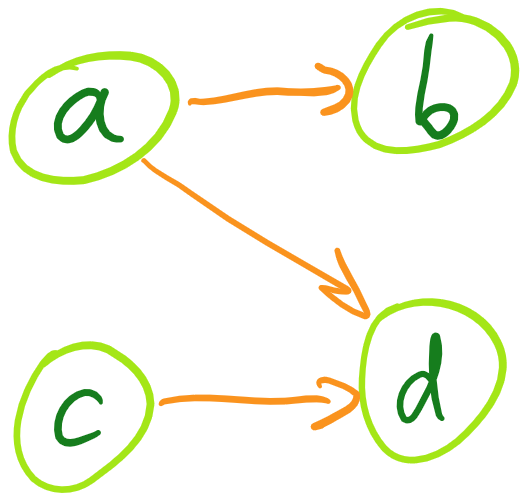
\includegraphics[scale=0.17]{images/graph_0_01.png}
		\pitem $V := \{a, b, c, d\}, E := \{(a,a), (b,b), (c,c)\}$\\
		\p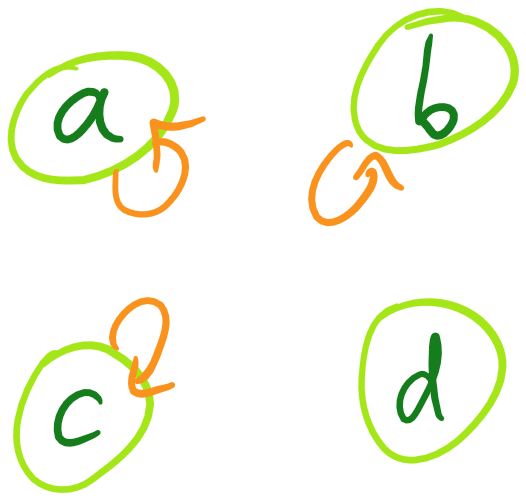
\includegraphics[scale=0.17]{images/graph_0_02.png}
		\pitem $V := \{a, b, c, d\}, E := \emptyset$\\
		\p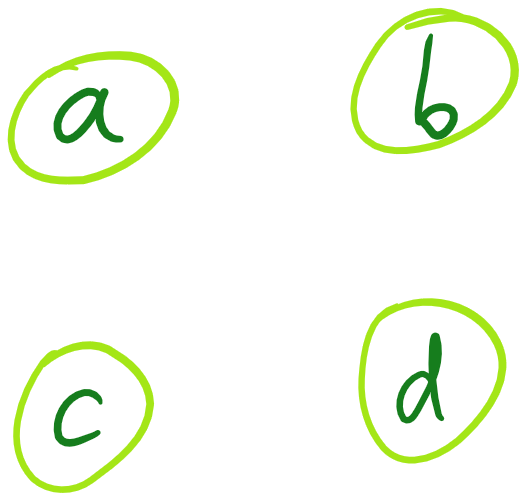
\includegraphics[scale=0.17]{images/graph_0_03.png}
	\end{itemize}
\end{frame}

\begin{frame}{Wann Angabe als Menge, wann als Visualisierung?}
	Wir verwenden gezeichnete Graphen und deren Definition als Mengen als äquivalent.
	
	\begin{itemize}
		\pitem $\{(a,b),(c,d),(a,d)\} = \{(a,b),(a,d),(c,d)\} \neq \{(b,a),(d,c),(d,a)\}$, also Kantenmenge mit unterschiedlichen Reihenfolgen darstellbar. Genauso die Knotenmenge.
	\end{itemize}

	\ip
	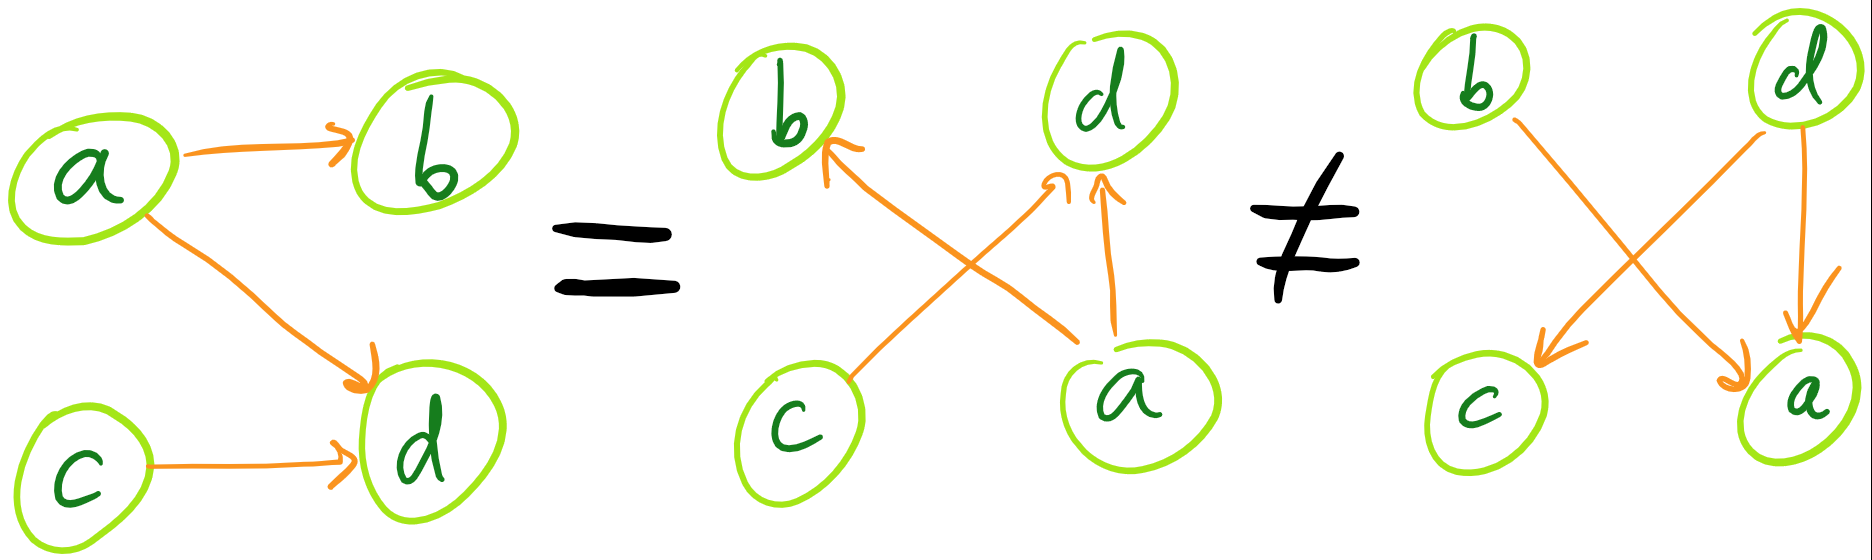
\includegraphics[scale=.3]{images/graph_1.png}
	
	\bp
	
	Es kann also in jedem Fall der Graph sowohl als ``Visualisierung'' oder als Menge angegeben werden, beide Varianten sind formal korrekt.
\end{frame}

\subsection{Praxisbeispiele}
% Hier bei allen Aussagen fragen, was die Tutanden als Ideen haben, wie man das als Graphenfrage formulieren kann
% Einige Sachen werden vorgegriffen (Wurzel, Knotengrad). Trotzdem fragen, Tutanden werden es vermutlich einfach komplizierter formulieren. Das so stehen lassen und erwähnen, dass darauf später genauer eingegangen wird.
% Dabei soll deutlich werden, dass konkrete Probleme in "die Sprache der Graphen" überführt werden kann und als bekanntes Problem gelöst werden kann

\begin{frame}{Praxisbeispiel: Soziales Netzwerk}
	\ip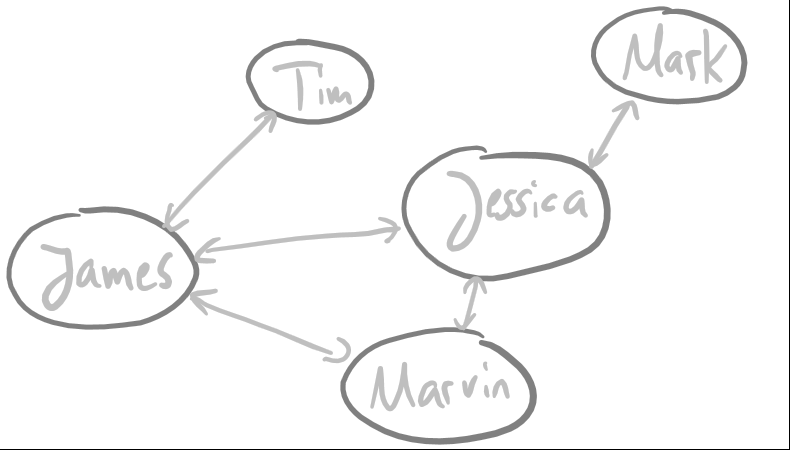
\includegraphics[scale=0.4]{images/graph_beispiel_socialnetwork.png}
	\begin{itemize}
		\pitem Ist Person $A$ direkt mit Person $B$ befreundet? \pause $\Leftrightarrow$ Gibt es eine Kante $(A,B)$?
		\pitem Ist Person $A$ über maximal 2 verschiedene Leute mit Person $B$ befreundet?\pause $\Leftrightarrow$  Gibt es einen Pfad von $A$ nach $B$ mit maximaler Länge 3?
		\pitem Wieviele Freunde hat Person $A$?\pause $\Leftrightarrow$ Welchen Grad hat Person $A \in V$?
	\end{itemize}
\end{frame}

\begin{frame}{Praxisbeispiel: Wie kommt man am schnellsten von $A$ nach $B$}
	\ip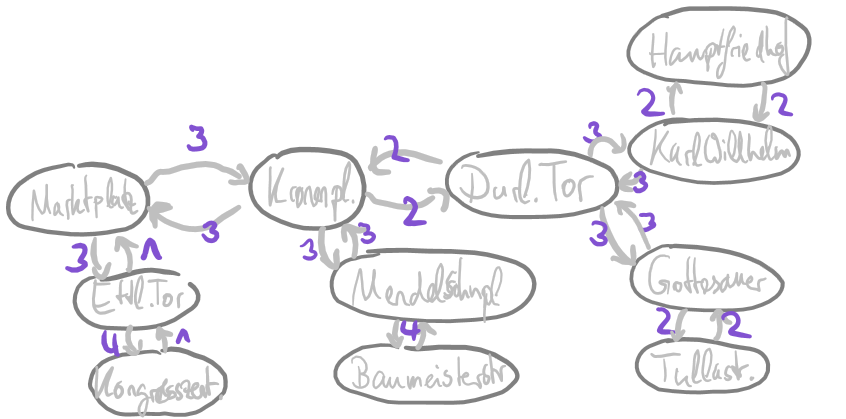
\includegraphics[scale=0.4]{images/graph_beispiel_kvv.png}
	\begin{itemize}
		\pitem Kantengewichtung: Jeder Kante wird eine Zahl $c \in \R$ zugewiesen.
		\pitem Wie lange dauert der kürzeste Weg von Kongresszentrum nach Hauptfriedhof? \pause $\Leftrightarrow$ Wie lang ist ein kürzester Pfad von Kongresszentrum nach Hauptfriedhof?
		\pitem Wo kommt man von Kronenplatz überall innerhalb von 5 Zeiteinheiten hin? \pause $\Leftrightarrow$ Für welche Orte $v \in V$ existiert ein Pfad $(Kronenplatz, ..., v)$ mit einer Länge von maximal 5?
	\end{itemize}
\end{frame}

\begin{frame}{Praxisbeispiel: Huffman-Bäume}
	\ip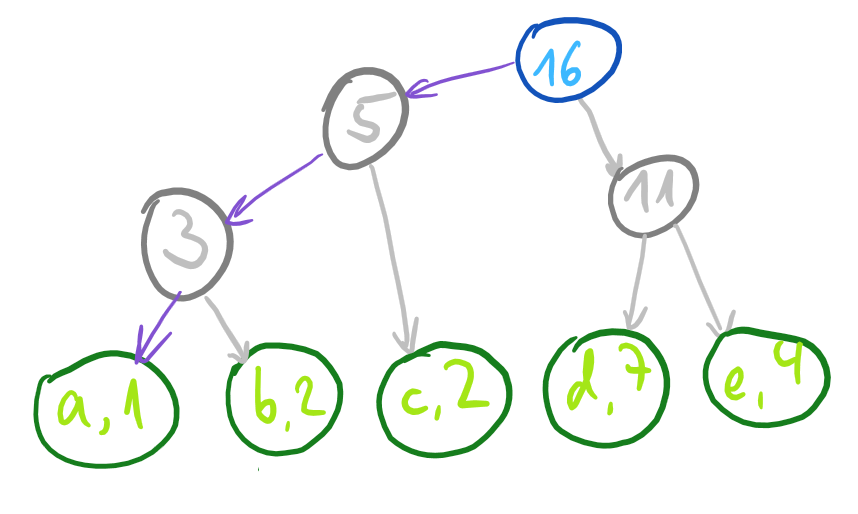
\includegraphics[scale=0.4]{images/graph_beispiel_huffman.png}
	\begin{itemize}
		\pitem Wie lang ist die Kodierung vom Zeichen $c$?\pause $\Leftrightarrow$ Wie lang ist der Pfad von Wurzel zu Knoten $c$? In diesem Fall $2$.
		\pitem Wie viele Zeichen werden kodiert? \pause $\Leftrightarrow$ Wie viele Knoten sind von der Wurzel erreichbar, die selbst keine ausgehenden Kanten haben? \pause $\Leftrightarrow$ Wie viele Blätter hat der Baum?
	\end{itemize}
\end{frame}


\subsection{Ungerichtete Graphen}
\begin{frame}{Ungerichtete Graphen}
	\begin{itemize}
		\pitem Bis jetzt\ip: Gerichtete Graphen\ip, dh. Kanten $(u,v)$ hatten eine Richtung von Knoten $u$ nach Knoten $v$.
	\end{itemize}

	\bp
	
	\begin{block}{Ungerichteter Graph}
		Ein ungerichteter Graph ist ein Graph\ip, dessen Kanten Mengen, und keine Tupel sind.
	\end{block}

	\bp
	
	\begin{itemize}
		\item Beispiel: Statt Kante $(u,v)$ jetzt Kante $\{u,v\} \pause = \{v, u\}$.
		\pitem Information über Richtung geht also verloren, Kanten verbinden nur noch Knoten, ohne sich zu merken, welcher Knoten Start und welcher Ziel ist.
	\end{itemize}
\end{frame}

\subsection{Begriffe}

\begin{frame}{Teilgraph}
	\begin{block}{Teilgraph}
		\ip Zu einem Graph $G := (V, E)$ \ip ist ein Teilgraph definiert \ip als $G' = (V', E')$\ip, falls gilt $V' \subseteq V$ und $E' \subseteq E$.
	\end{block}

	\bp	

	\begin{itemize}
		\item Beispiel: Sei $G := (V,E)$ mit $V := \{a,b,c,d,e,f\}$ und $E := \{(b,a),(b,f),(f,d),(e,f),(f,a),(e,b),(a,e),(f,c),(a,c),(c,a),(c,e)\}$
		\p\item Ist ein Graph mit $V_1:=\{a,c,d,e,f\}, E_1:= \{(a,c),(c,a),(a,e),(f,d)\}$ ein Teilgraph von $G$?
		\p\item Ist ein Graph mit $V_2:=\{d,f\}, E_2:= \{(f,d)\}$ ein Teilgraph von $G$?
		\p\item Ist ein Graph mit $V_3=E_3=\emptyset$ ein Teilgraph von $G$?
	\end{itemize}

	\bp
	
	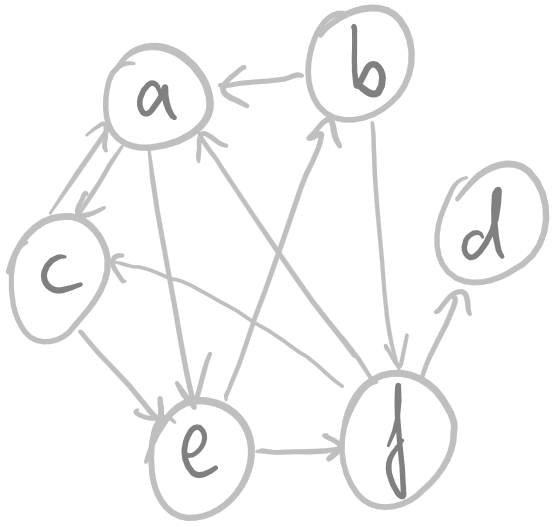
\includegraphics[scale=0.2]{images/graph_teilgraph_01.png}\ip
	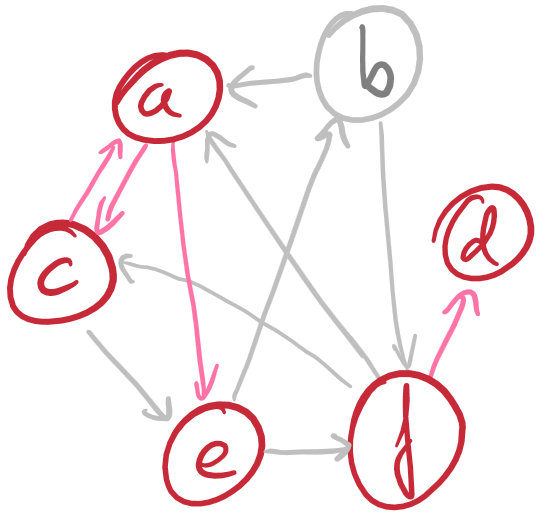
\includegraphics[scale=0.2]{images/graph_teilgraph_02.png}\ip
	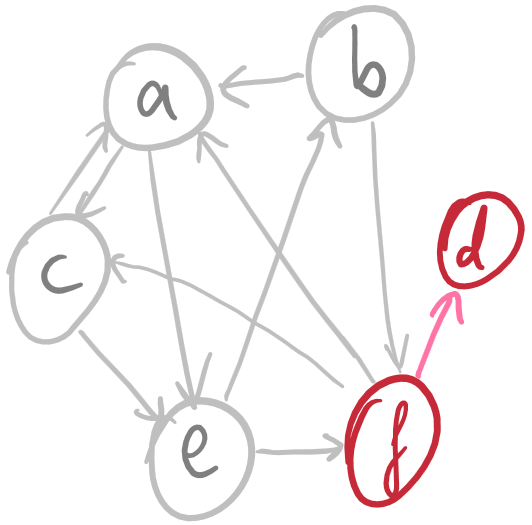
\includegraphics[scale=0.2]{images/graph_teilgraph_03.png}\ip
	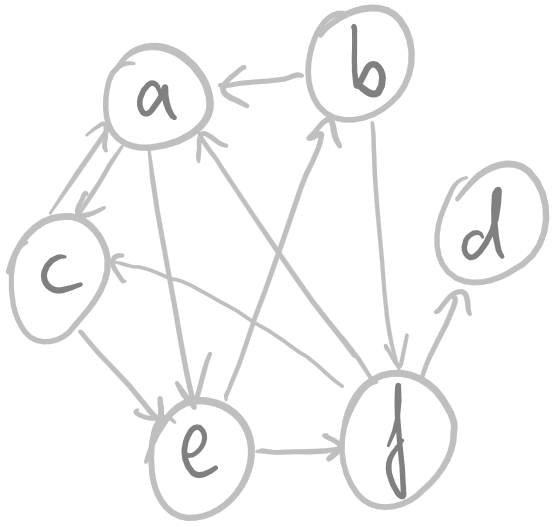
\includegraphics[scale=0.2]{images/graph_teilgraph_01.png} % Das ist technisch noch der letzte graph mit leeren kanten/knoten mengen
\end{frame}

\begin{frame}{Teilgraph}
	\begin{block}{Teilgraph}
		Zu einem Graph $G := (V, E)$ ist ein Teilgraph definiert als $G' = (V', E')$, falls gilt $V' \subseteq V$ und $E' \subseteq E$.
	\end{block}
	
	\begin{itemize}
		\item Beispiel: Sei $G := (V,E)$ mit $V := \{a,b,c,d,e,f\}$ und $E := \{(b,a),(b,f),(f,d),(e,f),(f,a),(e,b),(a,e),(f,c),(a,c),(c,a),(c,e)\}$
		\p\item Ist ein Graph mit $V_4:=\{a,b\}, E_4:= \{(f,d)\}$ ein Teilgraph von $G$?
		\p\item Ist ein Graph mit $V_5:=\{g,a\}, E_5:=\{(g,a),(a,g)\}$ ein Teilgraph von $G$?
		% Beides nicht.
	\end{itemize}
\end{frame}

\begin{frame}{Weg/Pfad}
	\begin{columns}
		\begin{column}{0.6\textwidth}
			\begin{block}{Pfad informell}
				Ein Pfad $(u,...,v)$ ist eine Aneinanderreihung von Knoten\ip, die jeweils mit Kanten verbunden sind\ip, sodass man über das \markGreen{traversieren} der Kanten vom Startknoten $u\in V$ zum Zielknoten $v\in V$ kommt.
			\end{block}
			
			\bp
			Anmerkung: Wenn man sich einen Knoten $x \in V$ merkt und eine Kante $(x,y) \in E$ traversiert, so gelangt man zu Knoten $y$.
			\bp
			
			\begin{block}{Pfad formell}
				Ein Pfad $P := (v_0, v_1, ..., v_n)$ der Länge $n$ \ip ist eine Permutation auf $V$ \ip, wobei gilt: \ip $\forall i \in \Z_n: (v_i, v_{i+1}) \in E$.
			\end{block}	
		\end{column}
		
		\begin{column}{0.4\textwidth}
			\bp
			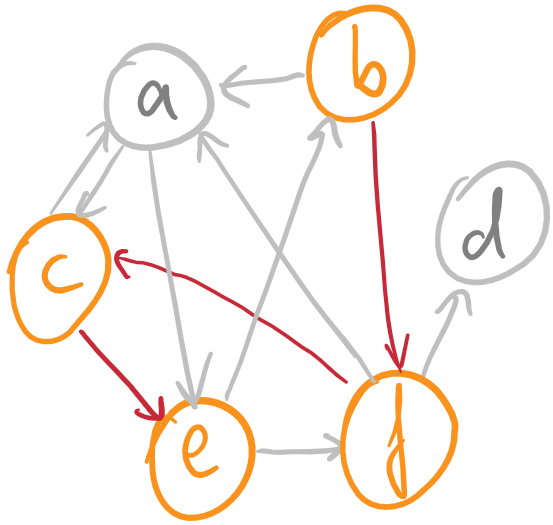
\includegraphics[scale=0.3]{images/graph_pfad.png}
			
			\ip Der Pfad $(b,f,c,e)$ ist ein möglicher Pfad von $b$ nach $e$ der Länge 3.
			
			\ip Gibt es noch andere solcher Pfade?
		\end{column}
	\end{columns}
\end{frame}

\begin{frame}{Zyklus}
	\begin{block}{Zyklus}
		\ip Ein Zyklus ist ein Pfad $(v_1, ..., v_n)$ mit $v_1 = v_n$.
	\end{block}
	\bp
	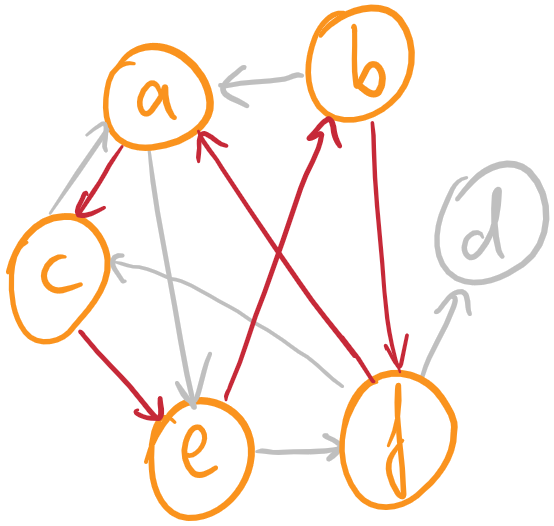
\includegraphics[scale=0.3]{images/graph_zyklus.png}
	
	\ip Der Pfad $(b,f,a,c,e)$ ist ein möglicher Zyklus.
	
	\ip Gibt es noch andere Zyklen?
\end{frame}

\begin{frame}{Zusammenhängend}

	% Jeweils Beispiele an der Tafel vormalen.

	\bp
	
	\begin{block}{Zusammenhängender Graph}
		Ein ungerichteter Graph heißt zusammenhängend, wenn gilt: $\forall u,v \in V \exists$ Pfad von $u$ nach $v$.
	\end{block}

	\bp

	\begin{block}{Stark zusammenhängender Graph}
		Ein gerichteter Graph heißt stark zusammenhängend, wenn gilt: $\forall u,v \in V \exists$ Pfad von $u$ nach $v$.
	\end{block}

	\bp
	
	\begin{block}{Schwach zusammenhängender Graph}
	Ein gerichteter Graph heißt schwach zusammenhängend, wenn der zugehörige ungerichteter Graph zusammenhängend ist.
	\end{block}
\end{frame}

\begin{frame}{Knotengrad}
	
	% Jeweils Beispiele an der Tafel vormalen.
	
	\begin{block}{Eingangsgrad}
		Der Eingangsgrad eines Knoten $u \in V$ ist definiert als: $d_{-}(u) := |\{(v, u) \in E: v \in V\}|$\ip, also die Anzahl der Kanten, die in den Knoten $u$ zeigen.
	\end{block}

	\bp 

	\begin{block}{Ausgangsgrad}
	Der Ausgangsgrad eines Knoten $u \in V$ ist definiert als: $d_{+}(u) := |\{(u, v) \in E: v \in V\}|$\ip, also die Anzahl der Kanten, die vom Knoten $u$ aus weg zeigen.
	\end{block}

	\bp
	
	\begin{block}{Grad}
		Der Grad eines Knoten $u$ ist definiert als: $d(u) := d_{+}(u) + d_{-}(u)$\ip, also die Anzahl der Kanten, über die $u$ verbunden ist.
	\end{block}
\end{frame}

\begin{frame}{Gerichtete Bäume}
	
	% Jeweils Beispiele an der Tafel vormalen.
	
	\begin{itemize}
		\pitem Kennt ihr schon: Huffman-Baum
	\end{itemize}

	\begin{block}{Gerichteter Baum}
	Ein gerichteter Baum ist ein \markGreen{schwach zusammenhängender kreisfreier} gerichteter Graph.	
	\end{block}

	\bp

	\begin{block}{Ungerichteter Baum}
		Ein ungerichteter Baum ist ein \markGreen{zusammenhängender kreisfreier} ungerichteter Graph.	
	\end{block}

	\bp

	\begin{itemize}
		\pitem Bäume haben immer einen Wurzelknoten, von dem alle anderen Knoten ausgehen.
		\pitem Ungerichtete Bäume \markBlue{können} mehrere Wurzeln haben.
		\pitem Knoten mit Grad 1 heißen Blätter.
	\end{itemize} 
\end{frame}



\begin{frame}{Randfälle}
	\begin{itemize}
		\pitem Wieviele Kanten kann ein Graph mit $n$ Knoten maximal haben? \pause $n^2$
		\pitem Wieviele Kanten kann ein schlingenfreier Graph mit $n$ Knoten maximal haben? \pause $n^2-n \p = n(n-1)$
		\pitem Wieviele Kanten kann ein ungerichteter Graph mit $n$ Knoten maximal haben? \pause $\frac{n(n-1)}{2}$
		\pitem Wieviele Kanten kann ein ungerichteter schlingenfreier Graph mit $n$ Knoten maximal haben? \pause $n + \frac{n(n-1)}{2} \p = \frac{n(n+1)}{2}$
	\end{itemize}
\end{frame}

\ifdefined\compileall
\else


\ifthenelse{\equal{\compiletype}{print}}
{

\begin{frame}{Informationen}
	
	\begin{columns}
		\begin{column}{0.5\textwidth}
			
			\begin{block}{Zum Tutorium}
				\begin{itemize}
					\item Lukas Bach
					\item Tutorienfolien auf: 
					\begin{itemize}
						\item \url{http://gbi.lukasbach.com}
					\end{itemize}
					\item Tutorium findet statt:
					\begin{itemize}
						\item Donnerstags, 14:00 - 15:30
						\item 50.34 Informatikbau, -107
					\end{itemize}
				\end{itemize}
			\end{block}
			
			\begin{block}{Mehr Material}
				\begin{itemize}
					\item Ehemalige GBI Webseite:
					\begin{itemize}
						\item \url{http://gbi.ira.uka.de}
						\item Altklausuren!
					\end{itemize}
				\end{itemize}
			\end{block}
			
		\end{column}
		\begin{column}{0.5\textwidth}
			
			\begin{block}{Zur Veranstaltung}
				\begin{itemize}
					\item Grundbegriffe der Informatik
					\item Klausurtermin:
					\begin{itemize}
						\item 06.03.2017, 11:00
						\item Zwei Stunden Bearbeitungszeit
						\item 6 ECTS für Informatiker und Informationswirte, 4 ECTS für Mathematiker und Physiker
					\end{itemize}
				\end{itemize}
			\end{block}
			
			\begin{block}{Zum Übungsschein}
				\begin{itemize}
					\item Übungsblatt jede Woche
					\item Ab 50\% insgesamt hat man den Übungsschein
					\item Keine Voraussetzung für die Klausur, aber für das Modul
				\end{itemize}
			\end{block}
			
		\end{column}
	\end{columns}
	
\end{frame}

}{}

\ifdefined\livebeamermode
	\begin{frame}
		
\includegraphics[width=\linewidth]{images/thatsall.png}
	\end{frame}
\fi

\end{document}

\fi